\documentclass[a4paper,12pt]{scrreprt}
\usepackage[left= 3cm,right = 3cm, bottom = 3.5 cm, top = 3 cm]{geometry}
\usepackage[onehalfspacing]{setspace}
\usepackage[utf8]{inputenc}
\usepackage{xfrac}
\usepackage{multirow}
\usepackage{graphicx}
\graphicspath{ {images/} }
\usepackage[ngerman]{babel}

\usepackage[backend=biber, style=numeric]{biblatex}
\addbibresource{biblatex.bib}

\def\workTitle{Der Titel meiner Diplomarbeit}
\def\studentFirstName{Max}
\def\studentLastName{Mustermann}
\def\studentId{Matrikelnummer}
\def\location{Institut / Universitätsklinik für .....}
\def\place{Wien}
\def\dateDay{01}
\def\dateMonth{01}
\def\dateYear{2020}
\def\advisorPreTitle{Dr.}
\def\advisoFirstName{Maximilia}
\def\advisorLastName{Musterfrau}
\def\advisorPosTitle{BSc. MSc.}
\def\assessorPreTitle{<Pre-Title>}
\def\assessorFirstName{<FirstName>}
\def\assessorLastName{<LastName>}
\def\assessorPosTitle{<Pos-Title>}

% define colors
\usepackage{color}
\definecolor{MDWblue}{RGB}{7, 29, 78}

% set font
\usepackage{mathptmx}
\setkomafont{disposition}{\bfseries}
\setkomafont{chapter}{\normalfont\huge}
\setkomafont{section}{\normalfont\Large}
\setkomafont{subsection}{\normalfont\large}

% set styles for headings
\RedeclareSectionCommand[
  %runin=false,
  afterindent=false,
  beforeskip=0pt,
  afterskip=\baselineskip]{chapter}
\RedeclareSectionCommand[
  %runin=false,
  afterindent=false,
  beforeskip=\baselineskip,
  afterskip=0.5\baselineskip]{section}
\RedeclareSectionCommand[
  %runin=false,
  afterindent=false,
  beforeskip=.75\baselineskip,
  afterskip=.5\baselineskip]{subsection}

% remove spacing between and around list items (enumerate and itemize)
\usepackage{enumitem}
\setlist{nosep}

\usepackage[
	pdftitle={\workTitle},
	pdfsubject={},
	pdfauthor={\studentFirstName \studentLastName},
	pdfkeywords={}
	pdftex=true, 
	colorlinks=true,
 	breaklinks=true,
	citecolor=black,
	linkcolor=black,	
	menucolor=black,	
	urlcolor=black
]{hyperref}

% Set meta data for PDF
\title{\workTitle}
\date{\dateYear-\dateMonth-\dateDay}
\author{\studentFirstName \studentLastName}

\begin{document}
\begin{titlepage}
    \newgeometry{left=0.4cm,right=0.4cm,bottom=1cm,top=1cm}
    \color{MDWblue}
    
\includegraphics[width=5.7cm]{uni-logo.png}

    \begin{center}
        \vspace*{1cm}

        \large Diplomarbeit \\
        \vspace{0.5cm}
        \Large\textbf{\workTitle}

        \vspace{3cm}

        \small zur Erlangung des akademischen Grades \\
        \large
        Doktor(in) der gesamten Heilkunde \\
        (Dr.med.univ.) \\
        \vspace{0.3cm}
        \small an der \\
        \large Medizinischen Universität Wien \\
        \vspace{0.3cm}
        \small
        ausgeführt am \dateDay.\dateMonth.\dateYear \\
        \location

        \vspace{1cm}

        unter der Anleitung von \\
        \advisorPreTitle\ \advisoFirstName\ \advisorLastName \if\advisorPosTitle\empty\else, \advisorPosTitle \fi \\
        Name der Co-BetreuerIn/des Co-Betreuers (nur 1 Angabe möglich, wenn vorhanden) \\

        \vspace{1cm}

        eingereicht von \\
        \textbf{\studentFirstName\ \studentLastName} \\
        \studentId

        \vfill

        \hfill\place, \dateDay.\dateMonth.\dateYear \hfill 
\includegraphics[width=3cm]{signature.png}\hspace*{\stretch{1}}
        \\[3.5cm]

    \end{center}
\end{titlepage}

\restoregeometry

\pagenumbering{Roman}

\newpage
\tableofcontents

\newpage
\chapter*{Kurzfassung}

Kurzfassung hier einfügen. Sie sollte nicht länger als eine Seite sein. Sie soll folgendermaßen strukturiert sein:

\begin{enumerate}
    \item kurze Darstellung von Hintergrund
    \item Problemstellung
    \item Rationale
    \item Methodik
    \item Verfahren
    \item Ergebnisse
    \item Schlussfolgerungen
\end{enumerate}

\newpage
\chapter*{Abstract}

Abstract goes here. It should not be longer than one page. The abstract should have the following structure:

\begin{enumerate}
    \item kurze Darstellung von Hintergrund
    \item Problemstellung
    \item Rationale
    \item Methodik
    \item Verfahren
    \item Ergebnisse
    \item Schlussfolgerungen
\end{enumerate}


\pagenumbering{arabic}

\chapter{Einleitung}
\label{ch:einleitung}

Darstellung von: Hintergrund, Fragestellung, Zielsetzung

\chapter{Material und Methoden}
\label{ch:methoden}

bei ethikpflichtigen Studien muss die EK-Kennzahl angegeben werden

\chapter{Resultate}
\label{ch:resultate}

Die nächsten Absätze können gelöscht werden und sollen nur eine Einleitung in Latex bieten.


\section{Strukturierung}
\label{ch:resultate:strukturierung}

\begin{tabular}{ l p{5.256cm} l }
    Code                   & Beschreibung                                                                     & Level der Überschrift \\ \hline
    \verb|\capter{Text}| & legt ein Kapitel an                                                              & 1                     \\
    \verb|\capter*{Text}| & legt ein Kapitel an, das nicht im Inhaltsverzeichnis gelistet wird               & 1                     \\
    \verb|\section{Text}| & legt einen Abschnitte an                                                         & 2                     \\
    \verb|\subection{Text}| & legt einen Unterabschnitt an                                                     & 3                     \\
    \verb|\subsubsection{Text}| & legt einen Unterunterabschnit an, der nicht im Inhaltsverzeichnis angeführt wird & 4
\end{tabular}

\section{Referenzieren}

Man kann auch auf vorherige Abschnitt verweisen (siehe \autoref{ch:resultate:strukturierung}). Wenn man sich nur die Zahl des Abschnittes ohne das Wort Kapitel/Abschnitt/\dots ausgeben lassen möchte, verwendet man~\ref{ch:resultate:strukturierung}. Die Tilde verhindert, dass die Referenz auf eine neue Zeile umbricht.


\section{Zitieren}

In der Datei \verb|biblatex.bib| befindet sich die Information über die Quellen, auf die man verweisen möchte. Diese Datei kann man sich von einem ``reference management program'' z.B. Zotero\footnote{\href{https://www.zotero.org/}{https://www.zotero.org/}} generieren lassen. Wichtig ist, dass sie im Format Biblatex --- nicht Bibtex --- vorliegt. Jetzt kann auf diese Quelle auf mehrere Arten verweisen:

\begin{itemize}
    \item Mit \verb|\cite{nachname_titel_jahr}| wird eine eckige Klammer mit der Laufnummer hinzugefügt~\cite{appelman_rose_1998}.
    \item Vielleicht möchte man nur die Namen der Autoren \citeauthor[hier noch ein Zusatz]{appelman_rose_1998} anführen.
    \item Der Titel lautet \citetitle{appelman_rose_1998}
    \item Geschrieben wurde das Paper \citeyear{appelman_rose_1998}.
    \item \dots
\end{itemize}


\section{Abbildung}

Ganz leicht können Abbildungen eingefügt werden (siehe \autoref{fig:meine-abbildung}). Der Zusatz in eckigen Klammern setzt die Position der Grafik. Eine Beschreibung der möglichen Werte findet man auf dem entsprechenden Knowledgebase Eintrag\footnote{\href{https://www.overleaf.com/learn/latex/Positioning\_of\_Figures}{https://www.overleaf.com/learn/latex/Positioning\_of\_Figures}} von Overleaf.

Mit \verb|\includegraphics{dateiname-in-graphics-folder}| wird die eigentliche \newline Grafik eingefügt. Der Zusatz in eckigen Klammern legt die Größe fest. Die Anweisung \verb|width=0.75\textwidth| setzt die Breite der Grafik auf \sfrac{3}{4} des Seiteninhalts.

\begin{figure}[h]
    \centering
    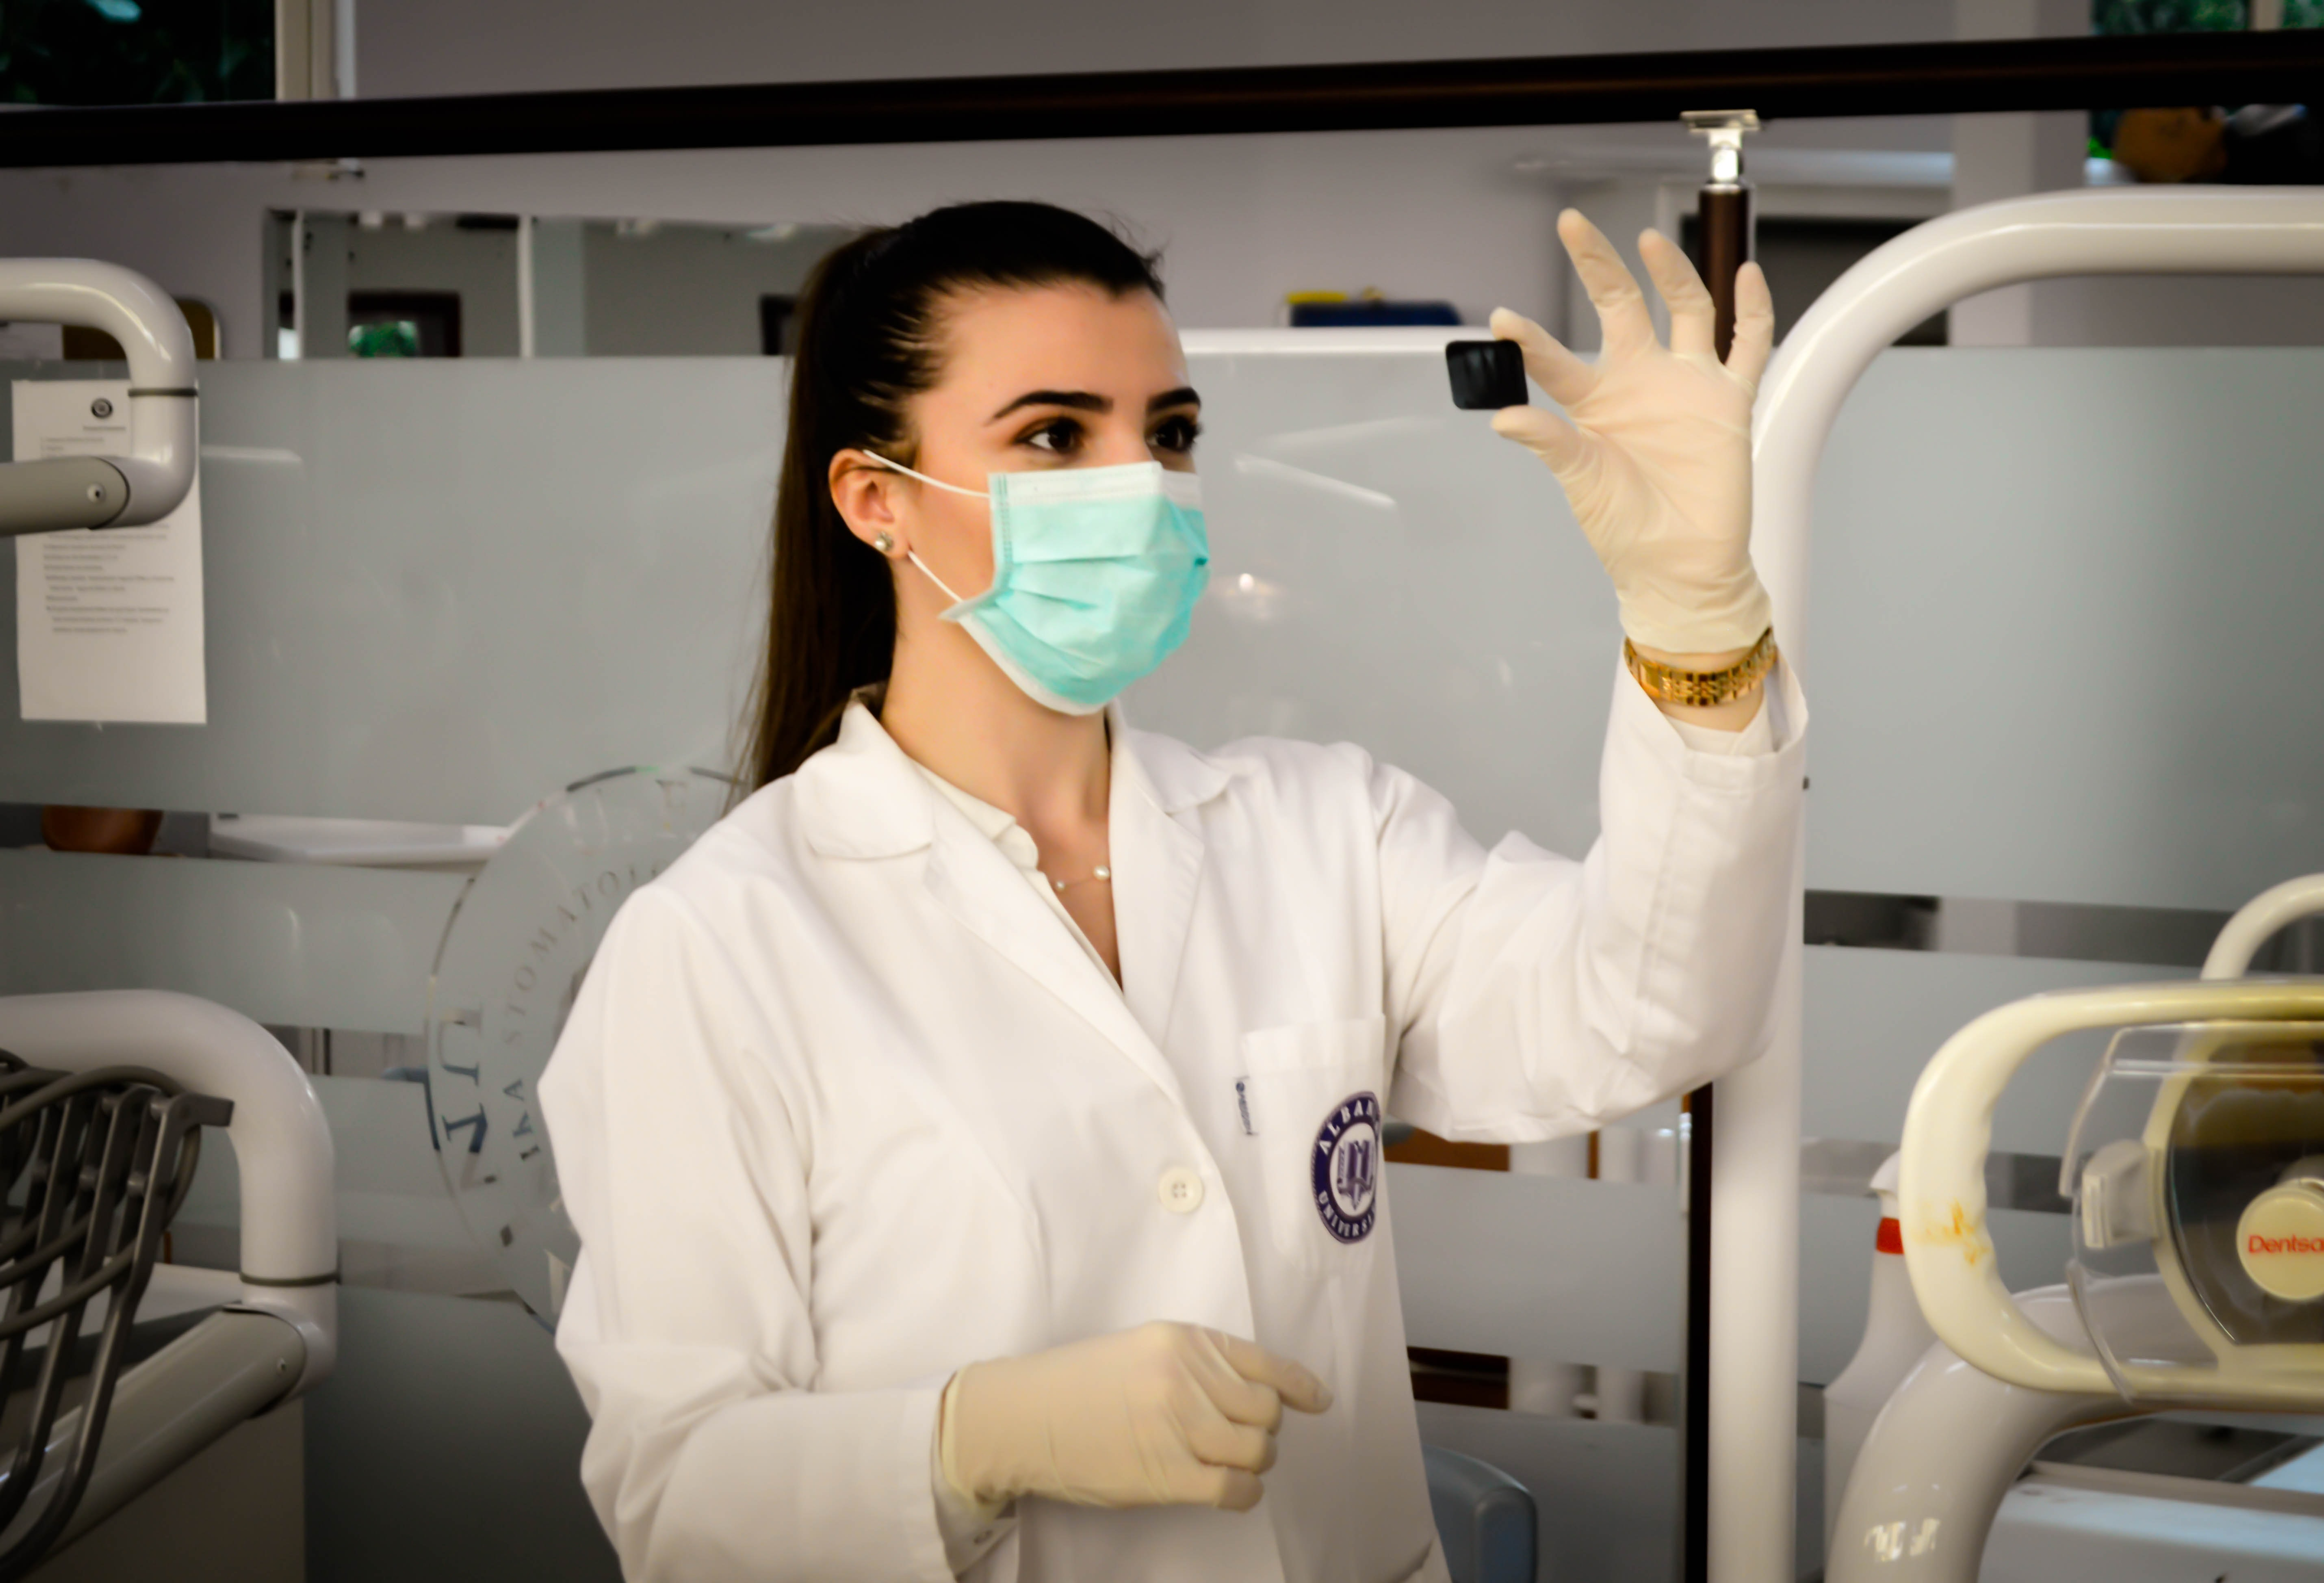
\includegraphics[width=0.75\textwidth]{ani-kolleshi.jpg}
    \caption{Meine erste Abbildung.}
    \label{fig:meine-abbildung}
\end{figure}


\newpage
\section{Tabellen}

Tabellen sind leider sehr unangenehm anzulegen. Die Website Tables Generator\footnote{\href{https://www.tablesgenerator.com/}{https://www.tablesgenerator.com/}} hilft allerdings. Ein Besipiel für eine simple Tabelle sieht man in \autoref{tab:meine-tabelle}.

\begin{table}[h]
    \centering
    \begin{tabular}{lll}
    \multicolumn{3}{l}{}                         \\
    id       & Vorname         & Nachname        \\ \hline
    1        & Max             & Mustermann      \\
    2        & Maximilia       & Musterfrau     
    \end{tabular}
    \caption{Meine erste Tabelle.}
    \label{tab:meine-tabelle}
\end{table}

\chapter{Diskussion}
\label{ch:diskussion}

Gegenüberstellung zu früheren Arbeiten, Schlussfolgerungen, Ausblick und eventuelle Anregungen für weiterführende Arbeiten

\chapter{Limitationen}
\label{ch:limitationen}


\newpage
\printbibliography

\newpage
\listoffigures

\newpage
\listoftables

\end{document}